\documentclass[a4paper,12pt]{report}

\usepackage{cmap}
\usepackage[T2A]{fontenc}
\usepackage[utf8]{inputenc}
\usepackage[english,russian]{babel}
\usepackage{listings}
\usepackage{amsmath}
\usepackage{float}
\usepackage{csquotes}
\usepackage{mathtools}

\usepackage{xcolor}
\usepackage{hyperref}

\usepackage{graphicx}
\graphicspath{ {./images/} }

\definecolor{dkgreen}{rgb}{0,0.6,0}
\definecolor{gray}{rgb}{0.5,0.5,0.5}
\definecolor{mauve}{rgb}{0.58,0,0.82}

\lstset{
    language=Python,                 % выбор языка для подсветки (здесь это С)
    basicstyle=\small\sffamily, % размер и начертание шрифта для подсветки кода
    numbers=left,               % где поставить нумерацию строк (слева\справа)
    numberstyle=\tiny,           % размер шрифта для номеров строк
    stepnumber=1,                   % размер шага между двумя номерами строк
    numbersep=5pt,                % как далеко отстоят номера строк от подсвечиваемого кода
    aboveskip=3mm,
    belowskip=3mm,
    showstringspaces=false,
    columns=flexible,
    captionpos=b, 
    basicstyle={\small\ttfamily},
    numbers=left,
    numberstyle=\tiny\color{gray},
    keywordstyle=\color{blue},
    commentstyle=\color{mauve},
    stringstyle=\color{dkgreen},
    breaklines=true,
    breakatwhitespace=true,
    tabsize=3
}

\title{Лабораторная работа №3\\Апериодические сигналы}
\author{Кобыжев Александр}
\date{\today}

\begin{document}

\maketitle
\tableofcontents
\listoffigures
\lstlistoflistings

\maketitle

\chapter{Упражнение 3.1}
\section{Пример утечки}

В данном упражнении нас просят открыть \texttt{chap03.ipynb}, запустить и прослушать примеры из блокнота. Также в задании прописано, что нужно заменить в примере с утечкой окно Хэмминга одним из окон, которое предоставляется \texttt{NumPy}. Для этого сначала рассмотрим пример утечки.

\begin{lstlisting}[caption=Пример утечки]
signal = thinkdsp.SinSignal(freq=440)
duration = signal.period * 30.25
wave = signal.make_wave(duration)
spectrum = wave.make_spectrum()

spectrum.plot(high=880)
thinkplot.config(xlabel='Frequency (Hz)')
\end{lstlisting}

\begin{figure}[H]
        \centering
        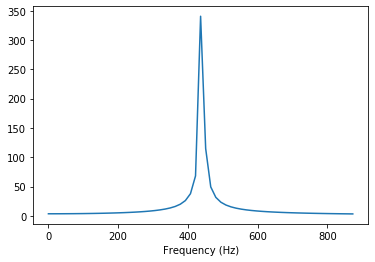
\includegraphics[width=0.75\textwidth]{lab3_fig1_1.png}
        \caption{Спектр утечки}
        \label{fig:lab3_fig1_1}
\end{figure}

\section{Замена окна Хэмминга}

Заменим окно Хэмминга на другие 4 окна.

\begin{lstlisting}[caption=Создание других окон]
for window_func in [np.bartlett, np.blackman, np.kaiser, np.hanning]:
    wave = signal.make_wave(duration)
    if window_func.__name__ == "kaiser":
        wave.ys *= window_func(len(wave.ys), 10)
    else:
        wave.ys *= window_func(len(wave.ys))
    spectrum = wave.make_spectrum()
    spectrum.plot(high=880, label=window_func.__name__)

thinkplot.config(xlabel='Frequency (Hz)', legend=True)
\end{lstlisting}

\begin{figure}[H]
        \centering
        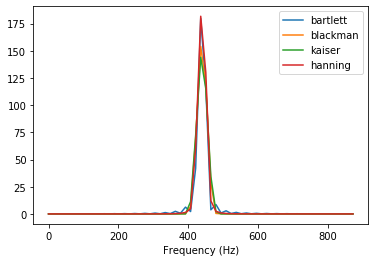
\includegraphics[width=0.75\textwidth]{lab3_fig1_2.png}
        \caption{Спектр созданных окон}
        \label{fig:lab3_fig1_2}
\end{figure}

Все четыре окна хорошо справляются с задачей уменьшения утечки.

\chapter{Упражнение 3.2}
\section{Написание класса SawtoothChirp}

Напишем класс \texttt{SawtoothChirp}, который переопределяет \texttt{evaluate} для генерации пилообразного сигнала.

\begin{lstlisting}[caption=Класс SawtoothChirp]
import math
PI2 = 2 * math.pi

class SawtoothChirp(thinkdsp.Chirp):
    def evaluate(self, ts):
        freqs = np.linspace(self.start, self.end, len(ts) - 1)
        dts = np.diff(ts)
        dphis = PI2 * freqs * dts
        phases = np.cumsum(dphis)
        phases = np.insert(phases, 0, 0)
        cycles = phases / PI2
        frac, _ = np.modf(cycles)
        ys = self.amp * frac
        return ys
\end{lstlisting}

\section{Проверка работоспособности}

После написания класса удостоверимся, что переопределённый метод действительно генерирует пилообразный сигнал с линейно увеличивающейся или уменьшающейся частотой путём прослушивания получившегося звука и рассмотрения спектрограммы.

\begin{lstlisting}[caption=Создание и воспроизведение звука]
signal = SawtoothChirp(start=300, end=900)
wave = signal.make_wave(duration=1, framerate=10000)
wave.apodize()
wave.make_audio()
\end{lstlisting}
    
На полученной спектрограмме эффект биений очевиден, а прослушав полученный до этого звук внимательно, можно даже их и услышать.

\begin{lstlisting}[caption=Спектрограмма звука]
sp = wave.make_spectrogram(1024)
sp.plot()
thinkplot.config(xlabel='Time (s)', ylabel='Frequency (Hz)')
\end{lstlisting}

\begin{figure}[H]
        \centering
        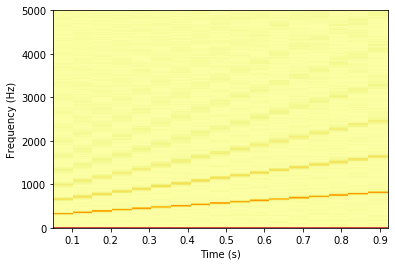
\includegraphics[width=0.75\textwidth]{lab3_fig2_1.png}
        \caption{Спектр сегмента звука}
        \label{fig:lab3_fig2_1}
\end{figure}

\chapter{Упражнение 3.3}

Поскольку основная частота колеблется от 2500 до 3000 Гц, я ожидаю увидеть что-то вроде высокой башни в этом диапазоне. Первая гармоника колеблется от 5000 до 6000 Гц, поэтому я ожидаю более короткую башню в данном диапазоне. Вторая гармоника колеблется от 7500 до 9000 Гц, поэтому я ожидаю что-то еще более короткое в этом диапазоне.

Другие гармоники повсюду накладываются друг на друга, поэтому я ожидаю увидеть некоторую энергию на всех других частотах. Эта распределённая энергия создает интересные звуки.

\begin{lstlisting}[caption=Создание сигнала]
signal = SawtoothChirp(start=2500, end=3000)
wave = signal.make_wave(duration=1, framerate=20000)
wave.make_audio()
\end{lstlisting}

Теперь посмотрим на получившийся спектр.

\begin{lstlisting}[caption=Визуализация спектра]
wave.make_spectrum().plot()
\end{lstlisting}

\begin{figure}[H]
        \centering
        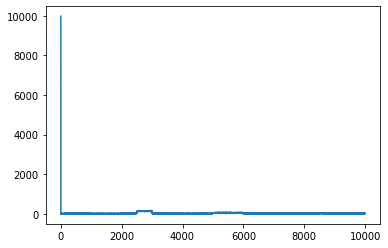
\includegraphics[width=0.75\textwidth]{lab3_fig3_1.png}
        \caption{Спектр созданного звука}
        \label{fig:lab3_fig3_1}
\end{figure}

Получился похожий график спектра, как я и предполагал, но нам мешает большая частота в самом начале, поэтому уберём её для более детального просмотра спектра звука.

\begin{lstlisting}[caption=Удаление частоты в начале]
cut_wave = wave.make_spectrum()
cut_wave.high_pass(10)
cut_wave.plot()
\end{lstlisting}

\begin{figure}[H]
        \centering
        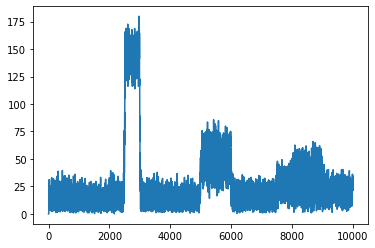
\includegraphics[width=0.75\textwidth]{lab3_fig3_2.png}
        \caption{Улучшенный спектр созданного звука}
        \label{fig:lab3_fig3_2}
\end{figure}

\chapter{Упражнение 3.4}

Для данного задания я нашёл в интернете глиссандо на скрипке.

\begin{lstlisting}[caption=Загрузка и прослушивание звука]
wave = thinkdsp.read_wave('411728__inspectorj__violin-glissando-ascending-a-h1.wav')
wave.make_audio()
\end{lstlisting}

Теперь рассмотрим спектрограмму звука.

\begin{lstlisting}[caption=Спектрограмма звука]
wave.make_spectrogram(512).plot(high=5000)
\end{lstlisting}

\begin{figure}[H]
        \centering
        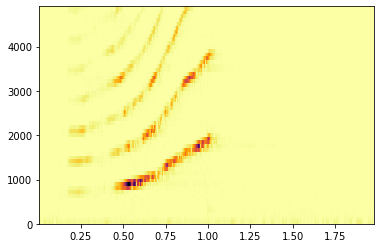
\includegraphics[width=0.75\textwidth]{lab3_fig4_1.png}
        \caption{Спектрограмма звука}
        \label{fig:lab3_fig4_1}
\end{figure}

Теперь мы можем наблюдать глиссандо.

\chapter{Упражнение 3.5}
\section{Создание класса}

Написанный класс представляет собой тромбоноподобный сигнал с переменной частотой.

\begin{lstlisting}[caption=Создание класса]
class TromboneGliss(thinkdsp.Chirp):
    def _evaluate(self, ts):
        l1, l2 = 1.0 / self.start, 1.0 / self.end
        lengths = np.linspace(l1, l2, len(ts)-1)
        freqs = 1 / lengths
        return self._evaluate(ts, freqs)
\end{lstlisting}

\section{Создание звука и его спектрограмма}

Создадим первую часть звука от C3 до F3, где C3 - 262 Гц, а F3 - 349 Гц.

\begin{lstlisting}[caption=Создание первой части звука]
low = 262
high = 349
signal = TromboneGliss(low, high)
wave1 = signal.make_wave(duration=1)
wave1.apodize()
wave1.make_audio()
\end{lstlisting}

Теперь создадим вторую часть звука от F3 до C3.

\begin{lstlisting}[caption=Создание второй части звука]
signal = TromboneGliss(high, low)
wave2 = signal.make_wave(duration=1)
wave2.apodize()
wave2.make_audio()
\end{lstlisting}

Затем соединим обе части в один полноценный звук.

\begin{lstlisting}[caption=Соединение двух частей звука]
wave = wave1 | wave2
wave.make_audio()
\end{lstlisting}

Теперь сделаем спектрограмму и расммотрим её.

\begin{lstlisting}[caption=Спектрограмма звука]
sp = wave.make_spectrogram(1024)
sp.plot(high=1000)
\end{lstlisting}

\begin{figure}[H]
        \centering
        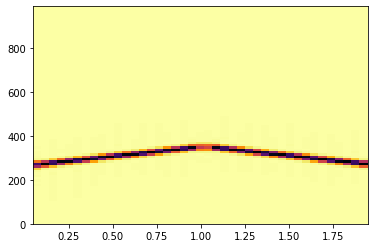
\includegraphics[width=0.75\textwidth]{lab3_fig5_1.png}
        \caption{Спектрограмма глиссандо на трамбоне}
        \label{fig:lab3_fig5_1}
\end{figure}

Глиссандо на тромбоне похоже на линейный чирп.

\chapter{Упражнение 3.6}

В интернете я нашёл гласные звуки, записанные женщиной, голос которой похож на голос бабы-яги из советских фильмов.

\begin{lstlisting}[caption=Загрузка и прослушивание звука]
wave = thinkdsp.read_wave('337631__anaphy__female-creak-vowels-a-e-i-o-u.wav')
wave.make_audio()
\end{lstlisting}

Теперь сделаем спектрограмму.

\begin{lstlisting}[caption=Создание спектрограммы]
wave.make_spectrogram(1024).plot(high=1000)
\end{lstlisting}

\begin{figure}[H]
        \centering
        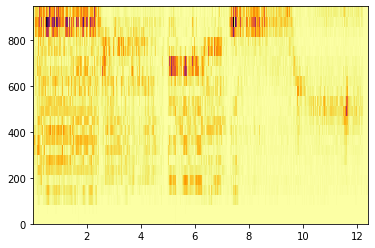
\includegraphics[width=0.75\textwidth]{lab3_fig6_1.png}
        \caption{Спектрограмма звука}
        \label{fig:lab3_fig6_1}
\end{figure}

Пики на спектрограмме называются формантами. В общем, гласные звуки различаются соотношением амплитуд первых двух формант относительно основного тона.

Мы можем увидеть форманты более чётко, выбрав сегмент во время \textquote{a}.

\begin{lstlisting}[caption=Спектр звука \textquote{a}]
high = 1000
thinkplot.preplot(5)

segment = wave.segment(start=0, duration=2)
segment.make_spectrum().plot(high=high)
\end{lstlisting}

\begin{figure}[H]
        \centering
        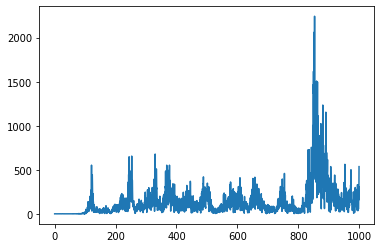
\includegraphics[width=0.75\textwidth]{lab3_fig6_2.png}
        \caption{Спектр звука \textquote{a}}
        \label{fig:lab3_fig6_2}
\end{figure}

Основная частота около 100 Гц. Следующие самые высокие пики находятся на 300 Гц и 900 Гц.

Выберем сегмент \textquote{e}.

\begin{lstlisting}[caption=Спектр звука \textquote{e}]
segment = wave.segment(start=2.5, duration=2)
segment.make_spectrum().plot(high=high)
\end{lstlisting}

\begin{figure}[H]
        \centering
        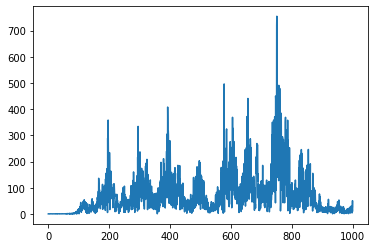
\includegraphics[width=0.75\textwidth]{lab3_fig6_3.png}
        \caption{Спектр звука \textquote{e}}
        \label{fig:lab3_fig6_3}
\end{figure}

Основная частота составляет 200 Гц. Следующие самые высокие пики находятся на 400 Гц и 600 Гц.

Выберем сегмент \textquote{i}.

\begin{lstlisting}[caption=Спектр звука \textquote{i}]
segment = wave.segment(start=4.5, duration=2.5)
segment.make_spectrum().plot(high=high)
\end{lstlisting}

\begin{figure}[H]
        \centering
        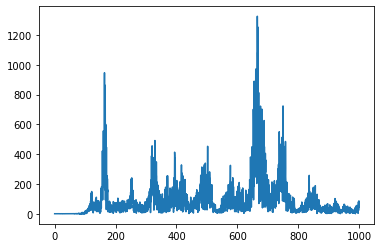
\includegraphics[width=0.75\textwidth]{lab3_fig6_4.png}
        \caption{Спектр звука \textquote{i}}
        \label{fig:lab3_fig6_4}
\end{figure}

Основная частота составляет 150 Гц. Следующие самые высокие пики находятся на 300 Гц и 750 Гц.

Это сегмент \textquote{o}:

\begin{lstlisting}[caption=Спектр звука \textquote{o}]
segment = wave.segment(start=7.5, duration=2)
segment.make_spectrum().plot(high=high)
\end{lstlisting}

\begin{figure}[H]
        \centering
        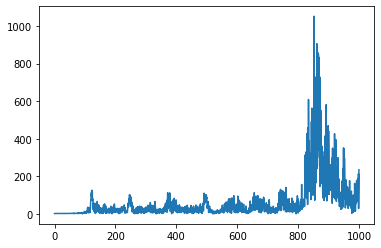
\includegraphics[width=0.75\textwidth]{lab3_fig6_5.png}
        \caption{Спектр звука \textquote{o}}
        \label{fig:lab3_fig6_5}
\end{figure}

Основная частота составляет 100 Гц. Следующие самые высокие пики находятся на частоте 900 Гц.

Это сегмент \textquote{u}:

\begin{lstlisting}[caption=Спектр звука \textquote{u}]
segment = wave.segment(start=10.2, duration=2)
segment.make_spectrum().plot(high=high)
\end{lstlisting}

\begin{figure}[H]
        \centering
        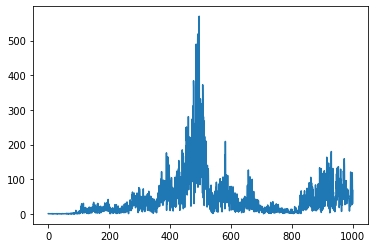
\includegraphics[width=0.75\textwidth]{lab3_fig6_6.png}
        \caption{Спектр звука \textquote{u}}
        \label{fig:lab3_fig6_6}
\end{figure}

Основной и самый высокий пик приходится на 500 Гц.

\chapter{Выводы}

Во время выполнения лабораторной работы получены навыки работы с апериодическими сигналами, частотные компоненты которых изменяются во времени, то есть практически все звуковые сигналы. Также рассмотрены спектрограммы - распространённый способ визуализации апериодических сигналов.

\end{document}